\setcounter{page}{1}


\section{Theorie}
Die Untersuchung einer Kettenschaltung von LC-Gliedern lässt sich mit der Analogie
zu einem eindimensionalen Festköper motivieren.
Der Versuch ermöglicht somit Einblicke in das Schwingverhalten eines
Festköpers. %redund

\subsection{Bestimmung der Schwingungsgleichungen für eine $LC$-Kette} %würde nicht $LC$
Die Schwingungsgleichung wird mit den Kirchhoffschen Regeln aufgestellt. %plural
Zunächst werden mittels der ersten Kirchhoffschen Regel die Ströme für ein Kettenglied $n$ %singular/plural
bestimmt (vgl. Abbildung \ref{fig:kettenglied}):

\begin{figure}
  \centering
  \includegraphics[width=0.8\textwidth]{bilder/stöme_und_spannnungen_lc.png}
  \caption{Kettenglied $n$.\cite{anleitung356}} %Zitat
  \label{fig:kettenglied}
\end{figure}

\begin{equation}
\label{eq:kircheins_lc}
I_n-I_{n+1}-I_{n,\map{quer}}=0
\end{equation}

Der Ansatz führt auf die Gleichung:

\begin{equation}
\label{eq:gleichung_lc}
-\omega^2CU\ua{n}+\frac{1}{L}\left(-U\ua{n-1}+2U\ua{n}-U\ua{n+1}\right)
\end{equation}
Diese wird durch
\begin{equation}
\label{eq:loesung_gleichung_lc}
U_n(t)=U_0 \map{e}^{j\omega t} \map{e}^{-jn\theta t}
\end{equation}
gelöst.
Es sei hierbei $\omega$ die Kreisfrequenz und $\theta$ die Phasenverschiebung, %kein komma nach theta, dafür nach phasenverschiebung
die durch ein Kettenglied verursacht wird.
Für die Kreisfrequenz ergibt sich die Dispersionsrelation:

\begin{equation}
\label{eq:kreisfrequenz_lc_glied}
\omega^2=\frac{2}{LC}\left(1-\cos(\theta)\right)
\end{equation}

Da \eqref{eq:kreisfrequenz_lc_glied} nur für endlich viele Kettenglieder definiert ist,
liegt $\omega$ maximal im Intervall: %-komma

\begin{equation}
\label{eq:menge_omega_lc_glied}
\omega\in\left[\,0,\frac{2}{\sqrt{LC}}\,\right)
\end{equation}

\subsection{Bestimmung der Schwingungsgleichungen für eine $LC_1C_2$-Kette}
Im Gegensatz zum vorherigen Kapitel, werden bei diesem Aufbau zwei unterschiedliche
Kondensatoren $C_1$ und $C_2$ verwendet. Die Kondensatoren werden
alternierend hintereinander geschaltet (vgl. Abbidldung \ref{fig:alternierende_kette}).

\begin{figure}
  \centering
  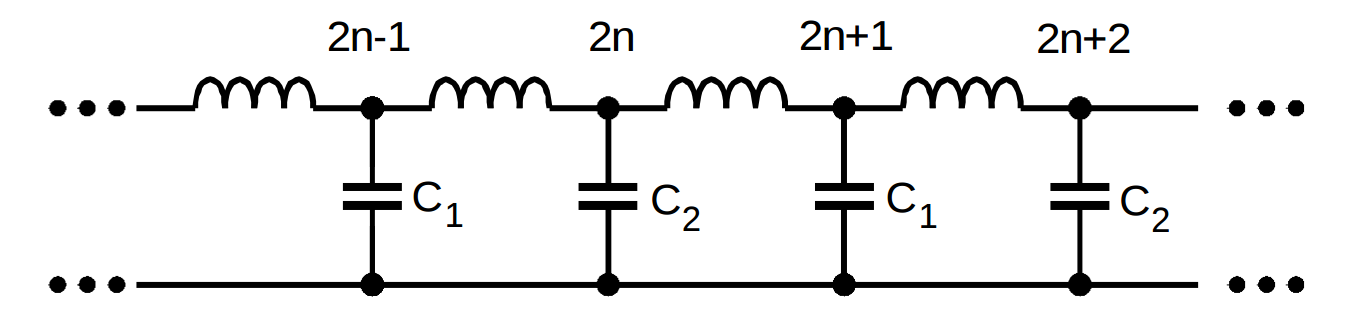
\includegraphics[width=0.8\textwidth]{bilder/alternierende_kette.png}
  \caption{$C_1C_2$ Kette.\cite{anleitung356}}
  \label{fig:alternierende_kette}
\end{figure}


Aufgrund dessen muss \eqref{eq:gleichung_lc} zu dem Gleichungssystem

\begin{align}
\label{eq:lc1c2_gleichungsy}
\begin{aligned}
-\omega^2C_1U_{2n+1}+\frac{1}{L}\left(-U_{2n}+2U_{2n+1}-U_{2n+2}\right)\\
-\omega^2C_2U_{2n}+\frac{1}{L}\left(-U_{2n-1}+2U_{2n}-U_{2n+2}\right)
\end{aligned}
\end{align}
erweitert werden.
Folglich ergeben sich die gleichen Lösungen wie bei \eqref{eq:gleichung_lc}
lediglich einmal mit $2n$ und einmal mit $2n+1$.
Durch Anwenden der Cramerschen Regel kann auf die Kreisfrequenz geschlossen werden: %Anwenden
\begin{equation*}
\omega^4-\omega^2\frac{2}{L}\left(\frac{1}{C_1}+\frac{1}{C_2}\right)+\frac{4}{L^2C_1C_2}\left(1-\cos^2(\theta)\right)=0
\end{equation*}
Diese Gleichung kann nach $\omega^2$ aufgelöst werden.
Das Resultat lautet: %doppelpunkt
\begin{equation}
\label{eq:omega_ceins_czwei}
\omega_{1,2}^{2}=\frac{1}{L}\left(\frac{1}{C_1}+\frac{1}{C_2}\right)\pm\frac{1}{L}\sqrt{\left(\frac{1}{C_1}+\frac{1}{C_2}\right)-\frac{4\sin^2(\theta)}{C_1C_2}}
\end{equation}

Es gibt also zwei verschiedene Kreisfrequenzen $\omega_1$ und $\omega_2$.
Trägt man beide Frequenzen in einem Diagramm auf, so ergeben sich %komma nach auf
zwei Kurven (vgl. Abbildung \ref{fig: dispersion_LC1C2}).
Zunächst soll die Lösung $\omega_2$ besprochen werden.
Wird diese bei $\theta=0$ betrachtet, ist ebenso $\omega=0$.
Mit der Näherung $\sin(\theta)\approx\theta$ ergibt sich dann

\begin{equation}
\label{eq:omega_2_lceins_czwei}
\omega_2\approx\sqrt{\frac{2}{L\left(C_1+C_2\right)}}\theta.
\end{equation}
Die Nullstelle von \eqref{eq:omega_2_lceins_czwei} liegt im Nullpunkt $\theta=0$.
Für $\theta>0$ wächst die Kurve monoton an.
Die Frequenz erreicht an der Stelle $\frac{\pi}{2}$, bei nicht Betrachtung der Näherung,
ein Maximum mit $\omega_2(\frac{\pi}{2})=\sqrt{\frac{2}{LC_1}}$.
 \newline
Hingegen beläuft sich bei $\omega_1$ die Lösung an der Stelle $\theta=0$ auf
\begin{equation}
\omega_1(0)\approx\sqrt{\frac{2(C_1+C_2)}{LC_1C_2}}
\label{eq: obere_grenfrequenz}
\end{equation}
Das Minimum von $\omega_1$ beträgt

\begin{equation}
\label{eq:max_omega_1_ceins_czwei}
\omega_1(\frac{\pi}{2})=\sqrt{\frac{2}{LC_2}}.
\end{equation}
Aufgrund des Unterschiedes der beiden Extrema, gibt es einen Frequenzbereich, in dem %aufgrund des Unterschiedes
die Kettenschaltung undurchlässig wird. Dieser ist auch in Abbildung \ref{fig: dispersion_LC1C2} %-auch
zu erkennen.

\subsection{Ausbreitungsgeschwindigkeit von Wellen in einer Kettenschaltung}
Bei einer Welle der Form \eqref{eq:loesung_gleichung_lc} %bei einer Welle der Form
ist die Ausbreitungsgeschwindigkeit unabhängig von der Phase %ist unabhängig von der Phase
\begin{equation*}
v\ua{ph}=\frac{\omega}{\theta}.
\end{equation*}
Es wird $v\ua{ph}$ als Phasengeschwindigkeit bezeichnet.
Die Zeitabhängigkeit der Phasengeschwindigkeit ist durch $\omega=\map{const}$
für alle Zeiten $t$ festgelegt. Wellen, die sich mit der Phasengeschwindigkeit
ausbreiten, sind aufgrund ihrer Unbeschränktheit in Raum und Zeit nicht zur %-komma
Informationsübermittlung geeignet. Hierzu benötigt man Wellenpakete, die sich
mit der Gruppengeschwindigkeit ausbreiten. Auf diese wird hier nicht eingegangen. %verb
Für eine LC-Kette ergibt sich als Phasengeschwindigkeit:

\begin{equation}
\label{eq:phasen_esc}
v\ua{ph}=\frac{\omega}{\theta}=\frac{\omega}{\arccos\!\left(1-\frac{1}{2}\omega^2LC\right)}
\end{equation}
Dabei geht die Phasengeschwindigkeit im Grenzfall in

\begin{equation*}
\lim_{\omega\to 0}v\ua{ph}=\frac{1}{\sqrt{LC}}
\end{equation*}

über.
\subsection{Der Widerstand einer unendlichen langen Kette}

Um den elektrischen Widerstand $R$ der Kettenschaltung zu bestimmen,
nutzt man die Kirchhoffschen Knotenregel (vgl. Abbildung \ref{fig:bestimmung_impe}) %-punkt
\begin{figure}
  \centering
  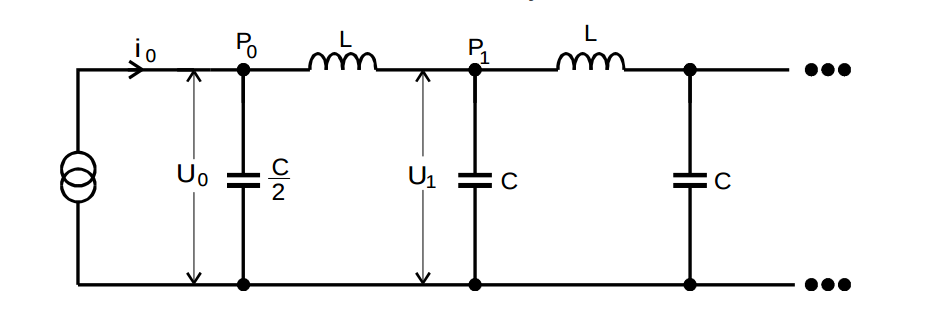
\includegraphics[width=0.8\textwidth]{bilder/eigenimpendanz.png}
  \caption{Spannungen un Ströme in der $LC$-Kette.\cite{anleitung356}}
  \label{fig:bestimmung_impe}
\end{figure}
\begin{equation*}
I_0 - \map{i}\omega\frac{C}{2}U_0+\frac{U_1-U_0}{\map{i}\omega L}=0.
\end{equation*}
Es sei $\map{i}$ das komplexe i. %merkse selber
Mit dem ohmschen Gesetz erhält man letztendlich %letztendlich

\begin{equation}
R(\omega)=Z\ua{LC}(\omega)=\sqrt{\frac{L}{C}}\frac{1}{\sqrt{1-\frac{1}{4}\omega^2LC}}.
\label{eq: wellenwiderstand_LC}
\end{equation}
Es ist üblich $R$ bzw. $Z$ als frequenzabhängigen Wellenwiderstand zu bezeichnen.
Für den Fall einer unendlich langen Kette ist der Widerstand rein reell, das bedeutet, %das bedeutet, dass es weder zu einer Phasenverschiebung noch zu einer Reflexion kommt.
dass es zu keiner Phasenverschiebung kommt.
Durch einen Abschlusswiderstand am Ende der Kette ist dieser Zustand auch bei einer endlichen Kette
realisierbar. Der Abschlusswiderstand muss dazu lediglich den Betrag $Z$ besitzen.
Obwohl $Z$ frequenzabhängig ist, kann für Frequenzen weit unterhalb der Grenzfrequenz $\nu\ua{G}$
\begin{equation*}
Z\ua{LC}\approx \sqrt{\frac{L}{C}}
\end{equation*}
angenommen werden. Für den Wellenwiderstand $Z\ua{LC_1C_2}$ der $\mathup{LC_1C_2}$-Kette gilt
in diesem Grenzfall:
\begin{equation}
  Z\ua{LC_1C_2} = \sqrt{\frac{2L}{C_1 + C_2}}
  \label{eq: Z_LC_1C_2}
\end{equation}

\subsection{Randverhalten einer endlichen Kette}
Je nach Endwiderstand $r$ kann es bei einer endlichen Kette
zu Wellenreflexionen kommen. In der Kette kommt es dann %zur Wellenreflexion oder zu Wellenreflexionen
zu Überlagerungen wie z.\,B. stehenden Wellen. %überarbeite diesen satz nochmal
Für die Spannungen bzw. Stromstärken am Kettenende (vgl. Bild \ref{fig:kettenende}) gilt:%gilt entweder beides plural oder beides singular

\begin{figure}
  \centering
  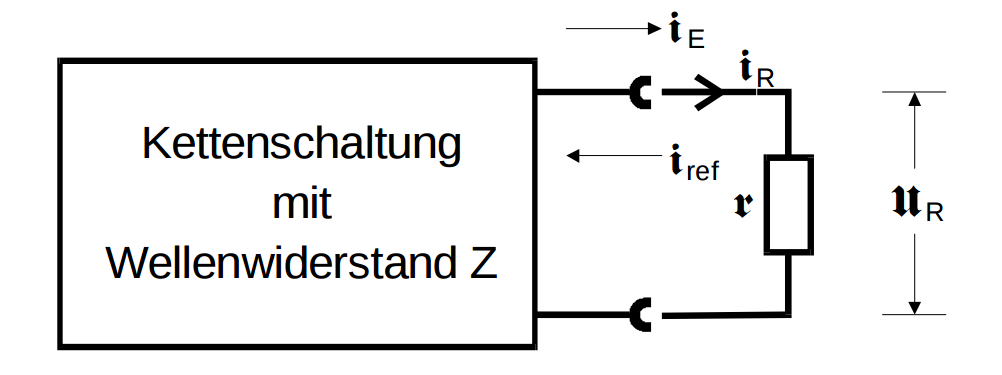
\includegraphics[width=0.6\textwidth]{bilder/wellenwiderstand.png}
  \caption{Kettenende.\cite{anleitung356}}
  \label{fig:kettenende}
\end{figure}

\begin{equation*}
U\ua{R}=U\ua{E}+U\ua{ref} \qquad I\ua{R}=I\ua{E}+I\ua{ref}
\end{equation*}

Es ist $U\ua{E}/I\ua{E}$ die Spannung/Stromstärke der einfallenden und $U\ua{ref}/I\ua{ref}$ die Spannung der reflektierten
Welle. Besitzt der elektrische Aufbau nun den Wellenwiderstand $Z$ so folgt nach dem
ohmschen Gesetz
\begin{equation*}
I\ua{E}=\frac{U\ua{E}}{Z} \qquad I\ua{ref}=\frac{U\ua{ref}}{Z}.
\end{equation*}
Somit ergibt sich das Verhältnis

\begin{equation*}
\frac{U\ua{ref}}{U\ua{e}}=\frac{r-Z}{r+Z}
\end{equation*}

Es gibt drei interessante Sonderfälle:

\renewcommand{\labelenumi}{\alph{enumi})}
\begin{enumerate}
\item{ $r=\infty$ (offenens Ende) \newline
Betrachten wir ein offenes Ende, so ist $U\ua{ref}=U\ua{e}$ und die Welle wird am Kettenende ohne Phasensprung reflektiert.} %offenes Ende,
\item{ $r=0$ (kurzgeschlossenes Ende) \newline
In diesem Fall ist $U\ua{ref}=-U\ua{e}$. Zusätzlich kommt es bei der reflektierten Welle zu einem Phasensprung von $\pi$.} %in diesem Fall
\item{ $r=Z$ \newline
Ist der Abschlusswiederstand genauso groß wie der Wellenwiderstand, entsteht keine Reflexion, folglich
ist $U_{ref}=0$. Somit kann eine unendlich lange Kette simuliert.}
\end{enumerate}

In allen anderen Fällen kommt es zu Teilreflexionen.
Bei den Fällen $r=\infty$ und $r=0$ erfolgt eine Totalreflexion.
Bildet sich im Schaltkreis eine stehende Welle aus, so bildet sich ein Spannungsbauch
genau dann aus, wenn %ch
\begin{equation}
\label{eq:spannungsbauch}
n\ua{max}\theta_k=k\pi \quad k=1,2,\dots,n\ua{max}.
\end{equation}
Es sind im Schwingkreis somit maximal $n\ua{max}$ stehende Wellen möglich. %s
Jede dieser stehenden Wellen besitz eine Frequenz $\omega_k$. %%überarbeite diesen satz nochmal
